\documentclass[a4paper,capchap,espacoduplo,normaltoc]{EPUSPclass/epusp_1.0.0}
%\usepackage[bookmarks,pdftex,a4paper,colorlinks=true,citecolor=black,urlcolor=blue,linkcolor=black,pdfpagemode=None]{hyperref}

% Main packages -----------------------------------------------------------
\usepackage[bookmarks,colorlinks=true,citecolor=black,urlcolor=blue,linkcolor=black,pdfpagemode=UseNone]{hyperref}
\usepackage[centertags]{amsmath}
\usepackage{amsfonts}
\usepackage{amssymb}
\usepackage{amsthm}
\usepackage[T1]{fontenc}
\usepackage[latin1]{inputenc}
%\usepackage[brazil]{babel}
\usepackage[english]{babel}
\usepackage[alf,abnt-repeated-author-omit=yes,abnt-title-command=yes,abnt-emphasize=bf]{abntex2cite} % \citeoption{abnt-emphasize=bf} --- need F11 to update bib file
\usepackage{url}
\usepackage{txfonts}
\usepackage{float}
\usepackage{booktabs} % for thicker lines in tables
%\usepackage{caption}
%\captionsetup[table]{labelsep=none}
%\usepackage[
%  labelfont={small,bf},
%  textfont={small},
%  labelsep=colon,singlelinecheck=false,format=plain,
%  parindent=1em]{caption}

% select font type -------------------------------------------------------
\usepackage{helvet} % close to arial
\renewcommand{\familydefault}{\sfdefault}
%\fontfamily{helvet}\selectfont %arial not working on unix
%\renewcommand{\rmdefault}{arial}

% Math -------------------------------------------------------------------
\newtheorem{theorem}{Theorem}{\bfseries}{\itshape}
\newtheorem{lemma}{Lemma}{\bfseries}{\itshape}
\newtheorem{definition}{Definition}{\bfseries}{\itshape}
\newtheorem{corollary}{Corollary}{\bfseries}{\itshape}
\newtheoremstyle{example}{\topsep}{\topsep}%
	{}%         Body font
	{}%         Indent amount (empty = no indent, \parindent = para indent)
	{\bfseries}% Thm head font
	{:}%        Punctuation after thm head
	{.5em}%     Space after thm head (\newline = linebreak)6
	{\thmname{#1}\thmnumber{ #2}\thmnote{ #3}}%         Thm head spec
\theoremstyle{example}
\newtheorem{example}{Example}
\newtheorem{assumption}{Assumption}{\bfseries}{\itshape}
\newtheorem{prop}{Proposition}{\bfseries}{\itshape}
\newtheorem{remark}{Remark}{\bfseries}{\itshape}

% Tables ------------------------------------------------------------------
\usepackage{longtable}
\usepackage{ltxtable}

% Graphics ----------------------------------------------------------------
\usepackage{scrextend}
\usepackage[pdftex]{graphicx}
%\graphicspath{{figures/}}
\DeclareGraphicsExtensions{.pdf,.jpeg,.png,.jpg}
\usepackage{pdfpages}

% Headers -----------------------------------------------------------------
\usepackage{fancyhdr}
\setlength{\headheight}{15pt}

% Others ------------------------------------------------------------------
%\pagestyle{fancyplain}
\renewcommand{\ABNTchaptermark}[1]{\markboth{#1}{}}
\renewcommand{\ABNTsectionmark}[1]{\markright{#1}{}}
\lhead{\fancyplain{}{\textit{\leftmark}}}
\chead{}
\rhead{\fancyplain{}{\thepage}}
\lfoot{}
\cfoot{}
\rfoot{}

\newcommand{\source}[1]{\\Source: {#1}}
\sloppy

% =============================================================================
\begin{document}
	%           #1          #2             #3           #4              #5
	%\autorPoli{firstnames}{firstinitials}{middlenames}{middleinitials}{surname}
	\autorPoli{Name}{N.}{}{}{Surname}

	\titulo{Your title goes here}

	\orientador{Prof. Dr. advisor name}

	\MiniPageText{Electrical Engineering (example)}

	\areaConcentracao{Systems Engineering (example)}

	\departamento{Departament of Control and Telecommunications Engineering (PTC)}

	\local{S�o Paulo}

	\data{2016}

	\capa{}

	\folhaderosto{}

	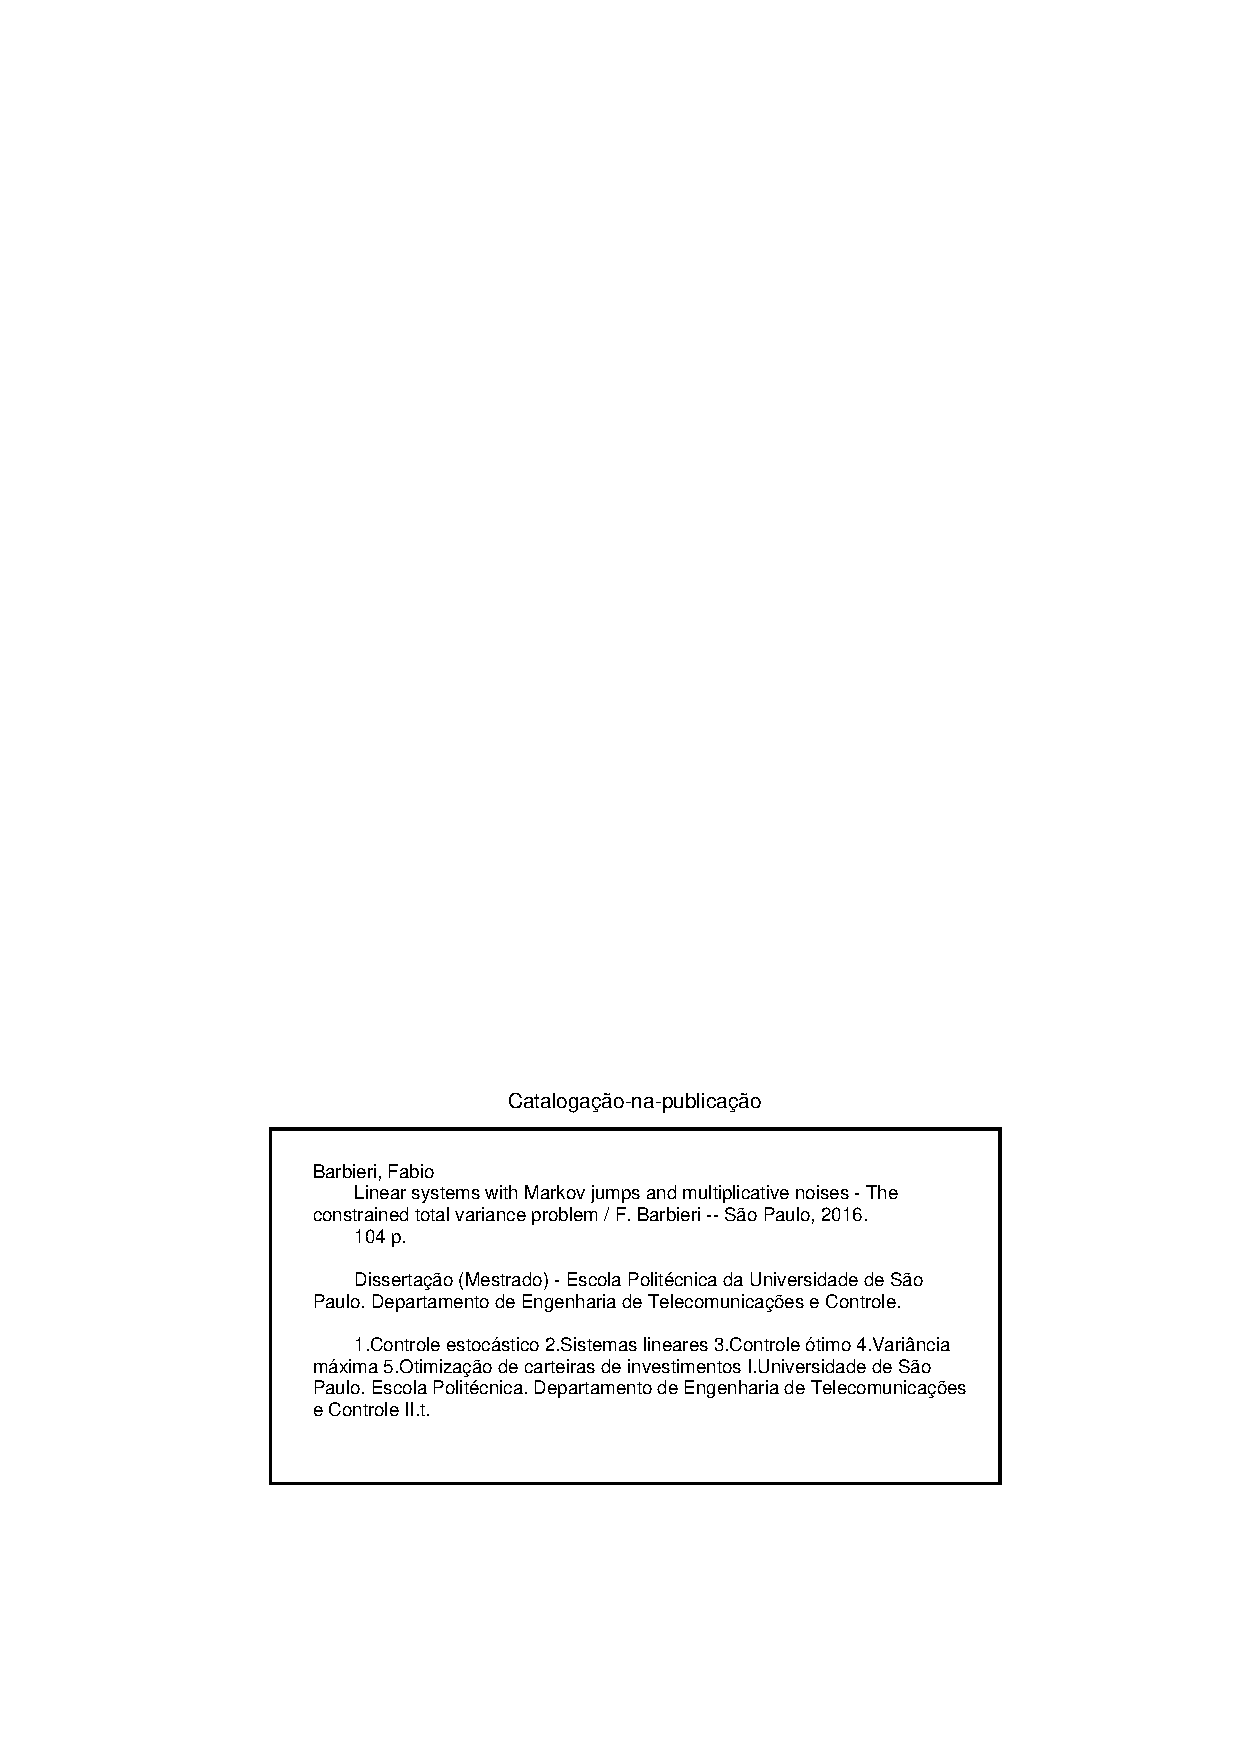
\includepdf[pages={1}]{figures/EPUSP-Catalogacao-na-Fonte}

	\pagenumbering{roman}

	\dedicatoria{To my family}

	\paginadedicatoria{}

	\begin{acknowledgement}
I thank all the people who...
\end{acknowledgement}


	\begin{resumo}

Neste trabalho, estudamos o problema...

\vspace{1\baselineskip}

\textbf{Palavras-chave:} Controle estoc\' astico. Sistemas lineares. Controle \' otimo. Vari\^ ancia m\' axima. Otimiza\c c\~ao de carteiras de investimento.

\end{resumo}


\begin{abstract}

In this work we study the...

\vspace{1\baselineskip}

\textbf{Keywords:} Stochastic control. Linear systems. Optimal control. Maximum variance. Portfolio optimization.

\end{abstract}


	\listoffigures

	\listoftables

	\begin{listofabbrv}{1000}
	\item [USP] Universidade de S\~ ao Paulo
	\item [CFS] Courtois-Finiasz-Sendrier
\end{listofabbrv}

	\begin{listofsymbols}{1000}
	\item [$\Delta(h)$] Assinatura di\' adica
\end{listofsymbols}

	\tableofcontents

	\pagenumbering{arabic}

	\chapter{Introdu\c c\~ ao} \label{chap:intro}
\pagestyle{fancyplain}


Here you should give the context, justifications...

Do yourself a favor and follow the structure guidelines in the file $Research\_structure\_guidelines.txt$.
It should make your life easier.

I left parts of my thesis as an example in my GitHub respository (\url{https://github.com/fbarbieri77}).
There you will find the syntax of a variety of commands about how to cite, include figures, tables, reference equations, formatting, etc.

In order to translate the default texts to another language you will need only to change the text at the end of the file "/EPUSPclass/definitions.tex" and change the language in the command line $usepackage[english]{babel}$ to $usepackage[brazil]{babel}$, for instance, in the main file.
Another option is to use the Portuguese version in my GitHub respository.

Have fun!!!


	\chapter{Revis\~ ao da Literatura} \label{chap:lit}


In your thesis you should update the file $/doc/bibliography.bib$ with your literature review papers.
Then you need to update the file $thesis\_main.bbl$ everytime you mention a new paper in the document.
I use TexMaker for linux and it is done by just pressing F11.

Examples of citation of one paper and multiple papers: We have studies that considered ... \cite{lim}, or cross terms ... \cite{luo}, or even studies that... \cite{liu,li2003,zhu2005}.

	\chapter{Methodology} \label{chap:method}

Introduction here...

\section{Notation and definitions} \label{notation}

	\chapter{Resultados} \label{chap:res}


	\chapter{Numerical examples} \label{chap:example}

In this chapter we illustrate the...

% --------------------------------------------------------------------###############
% --------------------------------------------------------------------###############
\section{Input parameters estimation} \label{s1}
% --------------------------------------------------------------------###############

In this section we will present...

% ---------------------------------------------------###############
\subsection{Data series} \label{ss1}
% ---------------------------------------------------###############

We considered the following Brazilian securities to be part of our portfolio and a proper index to compute the stochastic operation modes of our market (Table \ref{tab:assets}).
\begin{table}[h!] 
	\caption{List of assets.} 
	\centering
	%\setlength{\arrayrulewidth}{.03em}
	\begin{tabular}{*{3}{c}}
		\specialrule{1.5pt}{2pt}{2pt}
		\textbf{Ticker} \footnotemark[1]$^,$\footnotemark[2] & \textbf{Description} & \textbf{Sector}\\
		%Ticker $^{1,2}$ & Description & Sector\\
		\specialrule{0.3pt}{2pt}{2pt}
		IBOV & Bovespa index & - \\
		CDI & Interbank deposit rate & Fixed income \\
		EMBR3 & Embraer ON & Aviation OEM \\
		ITUB4 & Itau Unibanco PN & Banking \\
		PETR4 & Petrobras PN & Oil \& Gas \\
		VALE5 & Cia. Vale do Rio Doce PN & Metal \& Mining \\
		\specialrule{1.5pt}{2pt}{2pt}
%
	\end{tabular}
	\source{Author.}
	\label{tab:assets}
\end{table}
%
\footnotetext[1]{The CDI data source was the website \url{https://www.cetip.com.br}.}
%
\footnotetext[2]{The Ibovespa and risky assets' data source was the website \url{http://www.infomoney.com.br} which just make available data from the BMF \& Bovespa.}

The Bovespa Index (Ibovespa) is a total return index compiled as a weighted average of a theoretical portfolio of stocks and it is designed to gauge the stock market's average performance tracking changes in the prices of the more actively traded and better representative stocks of the Brazilian stock market.


The CDI is the overnight interbank deposit rate and it will be our proxy for the short term risk-free rate due to its high liquidity and low risk.
This rate is settled daily and, therefore, it is possible to capture the short term variations in the market expectations about the cost of money.

We chose risky securities from different industries in an attempt to decrease their correlation and improve our diversification and options during optimization.
Notwithstanding, all four risky assets figure among the most traded securities in the Bovespa stock exchange and, therefore, are very representative of that market.
The prices of the risky assets chosen were adjusted by dividends payments, stock splits, etc, in order to consider their proper historical performance.

All data series range from Jan-08-2001 to May-29-2015, covering 3.564 working days.
We contemplated a week as the standard interval of seven calendar days and reduced or increased this period to adjust for holidays.
Given the long Brazilian holidays like Carnival and near holidays like Christmas and $1^{st}$ of January, we reached a set of 740 weeks with a loss of around 12 weeks due to the accumulated adjustments over 14 years and 5 months.

We chose the weekly return and its smoothing, through a 12-week moving average, in order to reduce noise and improve the statistics results as suggested in \cite{valuation}.
All prices are in nominal Brazilian reais.


% ---------------------------------------------------###############
\subsection{Market's operation modes} \label{ss2}
% ---------------------------------------------------###############

The market's operation modes were defined using the Bovespa index depicted in Figure \ref{fig:ibovespa} below.
%
\begin{figure} [h!]
	\caption{Ibovespa index and its weekly average returns.}
	\centering
	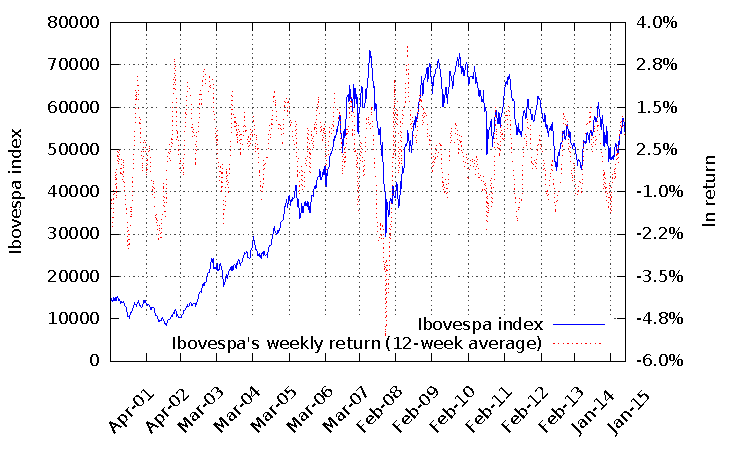
\includegraphics[width=5.5in,keepaspectratio]{figures/ibov}
	\source{Author.}
	\label{fig:ibovespa}
\end{figure}

There are some possible approaches to define modes and their probability transition matrix.
For instance, one could use econometric models, distributions adjustments as in \cite{oliveiraThesis}, or even simpler approaches without distribution adjustments as used in \cite{okimura2009}.

We will follow a mixed but still similar methodology as suggested in \cite{okimura2009} and \cite{oliveiraThesis}.
The main difference of our methodology regards the the criteria to split the market return's distribution, keeping the focus on other technical aspects of the resulting operation modes.

Our approach consists by first defining three regions around the market's 12-week average return, $R_{avg}$, each with width of one standard deviation, $\sigma_R$, multiplied by an adjustment factor, $a_f$.
Once we have the three middle regions with the same width, we will automatically be left with two regions at both extremes with no boundaries.
Thus, each region will have the following interval:
\begin{itemize}
	\item Region 1: $]-\infty ,\quad R_{avg} - 1.5 a_f \sigma_R]$
	\item Region 2: $]R_{avg} - 1.5 a_f \sigma_R ,\quad R_{avg} - 0.5 a_f \sigma_R]$
	\item Region 3: $]R_{avg} - 0.5 a_f \sigma_R ,\quad R_{avg} + 0.5 a_f \sigma_R]$
	\item Region 4: $]R_{avg} + 0.5 a_f \sigma_R ,\quad R_{avg} + 1.5 a_f \sigma_R]$
	\item Region 5: $]R_{avg} + 1.5 a_f \sigma_R ,\quad +\infty[$
\end{itemize}

We then set the adjustment factor in order to obtain extremes regions with enough data points to be considered statistically significant as defined below.
Thus, in our example, we proceeded with the Ibovespa's 12-week average returns distribution and defined each operation mode as described below.
\begin{description}
	\item[(i)] it shall have five operation modes considering scenarios of very low returns ("1 - Stress"), low returns ("2 - Low"), stable returns ("3 - Stable"), high returns ("4 - High"), and very high returns ("5 - Boom"); and
	\item[(ii)] every operation mode shall have more than 20 data points or at least 5\% of the total data points.
\end{description}

After computing the market's returns and their standard deviation, we set $a_f=1$ to obtain the intervals of each region as defined above.
This led to 55 and 41 data points in the two extreme scenarios respectively, providing them enough data points to be statistically significant as defined in item (ii) above.
 
The distribution and the operation modes' intervals obtained are shown in Figure \ref{fig:ibov_dist} and Table \ref{tab:modes} below.
%
\begin{figure} [h!]
	\centering
	\caption{Ibovespa's operation modes distributions.}
	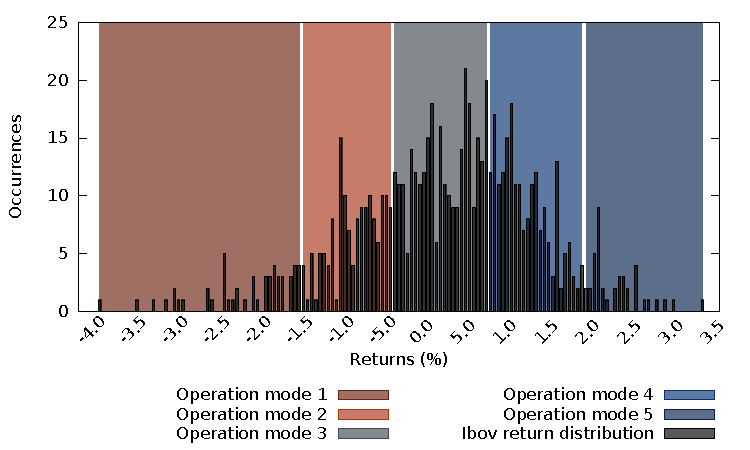
\includegraphics[width=6in,keepaspectratio]{figures/distr}
	\source{Author.}
	\label{fig:ibov_dist}
\end{figure}

%
\begin{table}[h!]
	\caption{Market operation modes.}
	\centering
	\begin{tabular}{*{6}{c}}
		\specialrule{1.5pt}{2pt}{2pt}
		\multicolumn{2}{c}{}& \multicolumn{2}{c}{Returns' range} & \multicolumn{2}{c}{}\\
		\specialrule{0.3pt}{2pt}{2pt}
		Mode & Description & $Min$ & $Max$ & Occurrence & Frequency \\
		\hline
		1 & Stress	& -$\infty$	& -1.5\%	& 55	& 7.4\%	\\
		2 & Low		& -1.5\%	& -0.4\%	& 158	& 21.4\%	\\
		3 & Stable	& -0.4\%	& 0.7\%		& 285	& 38.5\%	\\
		4 & High	& 0.7\%		& 1.9\%		& 201	& 27.2\%	\\
		5 & Boom	& 1.9\%		& +$\infty$	& 41	& 5.5\%	\\
		\specialrule{1.5pt}{2pt}{2pt}
	\end{tabular}
	\source{Author.}
	\label{tab:modes}
\end{table}

Once established the operation modes, we proceeded with the calculation of the  jumping frequencies to and from each mode.
%that each state changed or not to another mode.
The resulting transition probabilities is depicted in Table \ref{tab:transition}.
%
\begin{table}[h!]
	\caption{Operation modes transition matrix.}
	\centering
	\begin{tabular}{*{6}{c}}
		\specialrule{1.5pt}{2pt}{2pt}
		 & \multicolumn{5}{c}{Mode} \\
		 \specialrule{0.3pt}{2pt}{2pt}
		Mode 	& 1			& 2			& 3			& 4 		& 5\\
		\specialrule{0.3pt}{2pt}{2pt}
		1		& 70.9\%	& 29.1\%	& 0.0\%		& 0.0\%		& 0.0\%\\
		2		& 9.5\%		& 67.1\%	& 23.4\%	& 0.0\%		& 0.0\%\\
		3		& 0.4\%		& 12.0\%	& 70.0\%	& 16.9\%	& 0.7\%\\
		4		& 0.0\%		& 0.5\%		& 23.8\%	& 69.7\%	& 6.0\%\\
		5		& 0.0\%		& 0.0\%		& 2.4\%		& 31.7\%	& 65.9\%\\
		\specialrule{1.5pt}{2pt}{2pt}
	\end{tabular}
	\source{Author.}
	\label{tab:transition}
\end{table}

% ---------------------------------------------------###############
\subsection{Expected returns} \label{ss3}
% ---------------------------------------------------###############

In Table \ref{tab:returns} we show the annual average returns for each security given the operation modes obtained from the procedure described in the previous section.

Overall, the results followed the expected trend of higher returns for bullish markets and lower returns for bearish markets with the exception of the CDI asset in the Stress mode.
There, the CDI provided a higher return probably due to a higher demand for safe assets and/or expectation that the fixed income benchmark rate would increase to tackle the potential money outflow from Brazil.

%
\begin{table}[h!]
	\caption{Annual expected returns per market operation mode.}
	\centering
	\begin{tabular}{*{6}{c}}
		\specialrule{1.5pt}{2pt}{2pt}
		 & \multicolumn{5}{c}{Mode} \\
		 \specialrule{0.3pt}{2pt}{2pt}
		Security	& 1			& 2				& 3				& 4				& 5 \\
		\specialrule{0.3pt}{2pt}{2pt}
		Ibov	& -68.6\%		& -36.0\%		& 10.7\%		& 81.8\%		& 220.4\%\\
		CDI		& 14.6\%		& 12.4\%		& 13.0\%		& 13.9\%		& 18.8\%\\
		EMBR3	& -49.8\%		& -12.3\%		& 9.9\%			& 21.2\%		& 188.3\%\\
		ITUB4	& -56.3\%		& -26.1\%		& 22.6\%		& 86.5\%		& 143.3\%\\
		PETR4	& -70.3\%		& -43.0\%		& 16.1\%		& 101.5\%		& 136.5\%\\
		VALE5	& -53.5\%		& -29.5\%		& 23.5\%		& 72.9\%		& 137.1\%\\
		\specialrule{1.5pt}{2pt}{2pt}
	\end{tabular}
	\source{Author.}
	\label{tab:returns}
\end{table}

% ---------------------------------------------------###############
\subsection{Expected covariances} \label{ss4}
% ---------------------------------------------------###############

The expected covariances were calculated using the same set of modes as described previously and their resulting upper triangular matrices are depicted in Tables \ref{tab:cov1}, \ref{tab:cov2}, \ref{tab:cov3}, \ref{tab:cov4}, and \ref{tab:cov5} below.
%
Overall, we can notice that on average there is an increase in volatility from the Stable/High modes towards the Stress and Boom modes.
%
\begin{table}[h!]
	\caption{Annual expected covariances for mode 1.}
	\centering
	\begin{tabular}{*{7}{c}}
		\specialrule{1.5pt}{2pt}{2pt}
		 & \multicolumn{5}{c}{Security} \\
		 \specialrule{0.3pt}{2pt}{2pt}
		Security	& Ibov		& CDI			& EMBR3			& ITUB4			& PETR4			& VALE5 \\
		\specialrule{0.3pt}{2pt}{2pt}
		Ibov	& 0.002609		& -0.000006		& 0.002365		& 0.001177		& 0.002028		& 0.002984\\
		CDI		&				& 0.000016		& -0.000201		& 0.000016		& 0.000174		& 0.000264\\
		EMBR3	&				&		 		& 0.031981		& -0.000757		& -0.004895		& 0.001228\\
		ITUB4	&				&				& 		 		& 0.003384		& 0.000300		& -0.000247\\
		PETR4	&				&				& 		 		& 				& 0.012779		& 0.007728\\
		VALE5	&				&				& 		 		& 		 		& 				& 0.013388\\
		\specialrule{1.5pt}{2pt}{2pt}
	\end{tabular}
	\source{Author.}
	\label{tab:cov1}
\end{table}

\begin{table}[h!]
	\caption{Annual expected covariances for mode 2.}
	\centering
	\begin{tabular}{*{7}{c}}
		\specialrule{1.5pt}{2pt}{2pt}
		 & \multicolumn{5}{c}{Security} \\
		 \specialrule{0.3pt}{2pt}{2pt}
		Security	& Ibov		& CDI			& EMBR3			& ITUB4			& PETR4			& VALE5 \\
		\specialrule{0.3pt}{2pt}{2pt}
		Ibov	& 0.000444		& -0.000007		& -0.000038		& 0.000432		& 0.000463		& 0.000116\\
		CDI		&				& 0.000024		& -0.000188		& 0.000002		& 0.000116		& 0.000128\\
		EMBR3	&				&		 		& 0.010090		& 0.000527		& -0.001179		& 0.000204\\
		ITUB4	&				&				& 		 		& 0.002344		& 0.000159		& -0.000476\\
		PETR4	&				&				&		 		& 		 		& 0.009060		& 0.002828\\
		VALE5	&				&				&				& 		 		& 		 		& 0.004521\\
		\specialrule{1.5pt}{2pt}{2pt}
	\end{tabular}
	\source{Author.}
	\label{tab:cov2}
\end{table}

\begin{table}[h!]
	\caption{Annual expected covariances for mode 3.}
	\centering
	\begin{tabular}{*{7}{c}}
		\specialrule{1.5pt}{2pt}{2pt}
		 & \multicolumn{5}{c}{Security} \\
		 \specialrule{0.3pt}{2pt}{2pt}
		Security	& Ibov		& CDI			& EMBR3			& ITUB4			& PETR4			& VALE5 \\
		\specialrule{0.3pt}{2pt}{2pt}
		Ibov	& 0.000549		& -0.000001		& 0.000335		& 0.000684		& 0.000477		& 0.000506\\
		CDI		&				& 0.000030		& -0.000093		& 0.000053		& 0.000074		& 0.000065\\
		EMBR3	&				&		 		& 0.007809		& 0.000559		& -0.000724		& 0.000862\\
		ITUB4	&				&				& 		 		& 0.002799		& 0.000296		& 0.000643\\
		PETR4	&				&				&		 		& 		 		& 0.004692		& 0.000215\\
		VALE5	&				&				&				& 		 		& 		 		& 0.003980\\
		\hline
	\end{tabular}
	\source{Author.}
	\label{tab:cov3}
\end{table}

\begin{table}[h!]
	\caption{Annual expected covariances for mode 4.}
	\centering
	\begin{tabular}{*{7}{c}}
		\specialrule{1.5pt}{2pt}{2pt}
		 & \multicolumn{5}{c}{Security} \\
		 \specialrule{0.3pt}{2pt}{2pt}
		Security	& Ibov		& CDI			& EMBR3			& ITUB4			& PETR4			& VALE5 \\
		\specialrule{0.3pt}{2pt}{2pt}
		Ibov	& 0.000463		& 0.000004		& 0.000339		& 0.000388		& 0.000484		& 0.000218\\
		CDI		&				& 	0.000032	& 0.000115		& 0.000008		& -0.000015		& -0.000006\\
		EMBR3	&				&		 		& 0.007030		& 0.000209		& -0.000507		& -0.000134\\
		ITUB4	&				&				& 		 		& 0.001542		& 0.000374		& -0.000042\\
		PETR4	&				&				&		 		& 		 		& 0.004203		& 0.000030\\
		VALE5	&				&				&				& 		 		& 		 		& 0.005064\\
		\specialrule{1.5pt}{2pt}{2pt}
	\end{tabular}
	\source{Author.}
	\label{tab:cov4}
\end{table}

\begin{table}[h!]
	\caption{Annual expected covariances for mode 5.}
	\centering
	\begin{tabular}{*{7}{c}}
		\specialrule{1.5pt}{2pt}{2pt}
		 & \multicolumn{5}{c}{Security} \\
		 \specialrule{0.3pt}{2pt}{2pt}
		Security	& Ibov			& CDI			& EMBR3			& ITUB4			& PETR4		& VALE5 \\
		\specialrule{0.3pt}{2pt}{2pt}
		Ibov	& 0.000523		& -0.000037		& 0.000444		& 0.000798		& 0.000460		& 0.000280\\
		CDI		&				& 0.000030		& -0.000132		& -0.000137		& -0.000085		& -0.000185\\
		EMBR3	&				&		 		& 0.010195		& -0.000587		& -0.002001		& -0.000020\\
		ITUB4	&				&				& 		 		& 0.004025		& 0.002561		& 0.000753\\
		PETR4	&				&				&		 		& 		 		& 0.005077		& 0.001845\\
		VALE5	&				&				&				& 		 		& 		 		& 0.006882\\
		\specialrule{1.5pt}{2pt}{2pt}
	\end{tabular}
	\source{Author.}
	\label{tab:cov5}
\end{table}


% --------------------------------------------------------------------###############
% --------------------------------------------------------------------###############
\section{Simulations' results} \label{s2}
% --------------------------------------------------------------------###############

The objective in this section is to apply our results to a portfolio of financial securities, described by the System (\ref{eq:system}), and analyze its behavior when we impose a restriction on its total variance.
We first simulate a portfolio under different levels of $\alpha$ and then we provide a sensitivity analysis for different risk parameters $\beta$ and $\nu$.

% -------------------------------------###############
\subsection{Simulations for different levels of $\alpha$} \label{s_alpha}
% -------------------------------------###############

The investments are allocated among one reference asset and four risky assets.
The reference security will be the CDI and the risky assets will be EMBR3, ITUB4, PETR4, and VALE5.

We will use the parameters estimated previously to compute the matrices $\bar{A}$, $\tilde{A}$, $\bar{B}$, and $\tilde{B}$ as defined in Chapter \ref{chap:pm}.
The matrix $\bar{A}$ represents the reference asset's return and $\bar{B}$ represents the risky assets' returns.
The reference and risky assets' standard deviations matrices are associated with $\tilde{A}$ and $\tilde{B}$ respectively, where $\tilde{B}$ is obtained through the Cholesky decomposition of the covariance matrices. 

Note that, while the matrices $\bar{A}$, $\tilde{A}$, $\bar{B}$, and $\tilde{B}$ are given in percentage terms, the system's output, $y(t)$, the portfolio's value, $x(k)$, and the control policy, $u(k)$, are all defined in monetary terms, $R\$$ in our case.

Our investment horizon is set at $T=20$ weeks and the initial wealth as $x(0) = 1$ monetary unity.
The Markov chain will have $N=5$ operation modes starting at $\theta(0) = 3$ and its transition matrix is defined as in Table \ref{tab:transition}.
The mutual correlation matrix between our multiplicative noises is defined as $\rho_{s1,s2}(k) = I$.

The weekly expected returns and standard deviations are then obtained through Tables \ref{tab:returns}, \ref{tab:cov1}, \ref{tab:cov2}, \ref{tab:cov3}, \ref{tab:cov4}, and \ref{tab:cov5} depending on the mode provided by the Markov chain on every $k=0, \cdots, T-1$.

We then define four scenarios to run our model according to Table \ref{tab:scenarios} below.
%
\begin{table}[h!]
	\caption{Scenarios definition.}
	\centering
	\begin{tabular}{*{6}{c}}
		\specialrule{1.5pt}{2pt}{2pt}
			\multicolumn{2}{c}{}& \multicolumn{3}{c}{Risk parameters} & Restriction \\
			\multicolumn{2}{c}{}& \multicolumn{3}{c}{$t = 1,2, \dotsc, 20$} & \textit{(R\$)} \\
	 	\specialrule{0.3pt}{2pt}{2pt}
			Scenario & Problem applied	& $\nu(t)$	& $\xi(t)$	& $\beta(t)$	&  $\alpha$ \\
		\specialrule{0.3pt}{2pt}{2pt}
			A		 & $PU(\nu,\xi)$			& 1.0		& 1.0		& -				& - \\
			B		 & $PC(\nu,\beta,\alpha)$	& 1.0		& -			& 1.0			& 50.0 \\
			C		 & $PC(\nu,\beta,\alpha)$	& 1.0		& -			& 1.0			& 20.0 \\
			D		 & $PC(\nu,\beta,\alpha)$	& 1.0		& -			& 1.0			& 0.1 \\
		\specialrule{1.5pt}{2pt}{2pt}
	\end{tabular}
	\source{Author.}
	\label{tab:scenarios}
\end{table}

In the first scenario we solve the unconstrained problem, $PU(\nu,\xi)$, while in the other three scenarios we solve the $PC(\nu,\beta,\alpha)$ problem for different restrictions on the total variance, $\alpha$.
In this way we can observe how the output, variance, and control policy change from an unconstrained problem to a constrained one with a decreasing total variance boundary.

The first scenario problem, $PU(\nu,\xi)$, is solved by following the steps as described in Section \ref{remark:uk}. %, Chapter \ref{chap:form}. 	

The $PC(\nu,\beta,\alpha)$ problem is solved following the same steps described in Section \ref{remark:uk}, however, we now take the restriction $\alpha$ into consideration by computing $\xi$ using Equation (\ref{tPC3:e1}) and $\beta$ as defined in Table \ref{tab:scenarios}.
With this calculated $\xi$, we obtain $\lambda$ from Equation (\ref{PU:lambda}) and the optimal control policy of $PC(\nu,\beta,\alpha)$ using Equation (\ref{u_k}). 

% ###
The risk parameters $\nu(t)$, $\xi(t)$, and  $\beta(t)$ were assumed to be equal to one in every time step.
Thereby, by attributing the same risk relevance among all time steps related to both parameters,
we are assuming that the investor has no risk bias towards neither the system's output nor its variance over time.
Different risk aversion characteristics would lead to different relative weights among the elements of 
the risk parameters. %$\nu(t)$, $\xi(t)$, and  $\beta(t)$.
In order to show how the results may change with changes in risk perceptions, we provided a sensitivity analysis for our $PC(\nu,\beta,\alpha)$ problem by changing $\beta$ and $\nu$ in Section \ref{specific} below.

Finally, after 10,000 simulations, we obtain the results shown in the following charts and Table \ref{tab:results}.
%
\begin{table}[h!]
	\caption{Resulting total variance and other parameters for $PC(\nu,\beta,\alpha)$ problem.}
	\centering
	\begin{tabular}{*{7}{c}}
		\specialrule{1.5pt}{2pt}{2pt}
		Scenario 
			& $r_1$		& $r_2$		& $r_3$		& $f(\beta,\alpha)$	& $\xi(t)$
											& $\sum_{t=1}^{T}\nu(t)Var[y^u(t)]$ \\
		\specialrule{0.3pt}{2pt}{2pt}
		A	& -			& -			& -			& -					& 1.000	& 118.2\\
		B	& 118.2	& -3.6e-15	& -50		& 0.651				& 0.651	& 50\\
		C	& 118.2	& -3.6e-15	& -20		& 0.411				& 0.411	& 20\\
		D	& 118.2	& -3.6e-15	& -0.1		& 0.029				& 0.029	& 0.1\\
		\specialrule{1.5pt}{2pt}{2pt}
	\end{tabular}
	\source{Author.}
	\label{tab:results}
\end{table}

As expected, for all last three scenarios, the solution of $PC(\nu,\beta,\alpha)$ problem led to $\sum_{t=1}^{T}\nu(t)Var[y^u(t)] = \alpha$ by finding a proper $f(\beta,\alpha)$.

The output of the system is shown in Figure \ref{fig:output} below where we can see that an imposed lower total variance led to lower returns in every time step.
%
\begin{figure} [h!]
	\caption{System's output for all scenarios.}
	\centering
	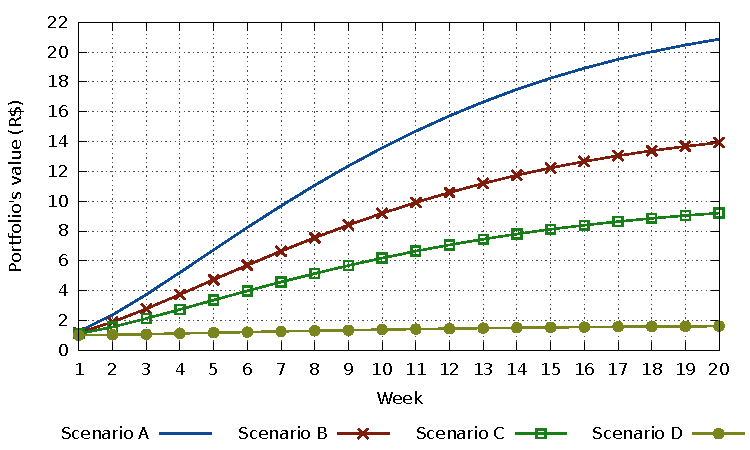
\includegraphics[width=6in,keepaspectratio]{figures/y_t}
	\source{Author.}
	\label{fig:output}
\end{figure}

The variance over time for all scenarios is shown in Figure \ref{fig:var1}.
In all cases we can see that the shape of the curve smooths gradually as the restriction $\alpha$ decreases, which means that although our restriction targets the total variance, we are able to lower the variance accordingly in each step providing that we have the same risk input parameters in each scenario.
%
\begin{figure} [h!]
	\caption{System's output variance for all scenarios.}
	\centering
	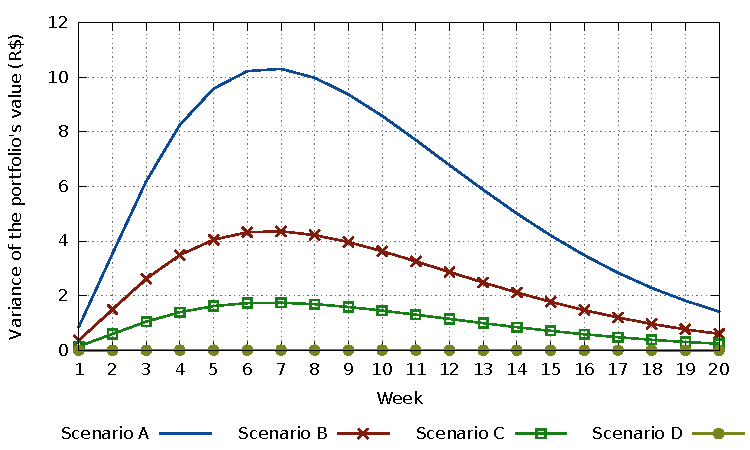
\includegraphics[width=6in,keepaspectratio]{figures/var_1}
	\source{author.}
	\label{fig:var1}
\end{figure}


The control policies shown in Figures \ref{fig:u1}, \ref{fig:u2}, \ref{fig:u3}, and \ref{fig:u4} reveal that the introduction of a lower restriction on the variance forces the solution to distribute a lower volume in all risky assets while keeping almost the same relative allocation among them.

On the other hand, the lower volume in the risky assets is now counter-balanced by a reduction in the borrowings using the CDI.
Notice that the CDI changes from an instrument of leverage to an investment in the later periods in scenario D, (Figure \ref{fig:u4}.

The results suggest that the proportional optimal allocation is barely affected by the total variance restriction and that the minimization of the total variance is done by managing the allocation in the risk-free asset.

In the limit, we will obtain a portfolio almost fully allocated in the CDI as our restriction $\alpha$ approaches zero.
The only reason it does not reaches 100\% allocation in the CDI is because we have considered the correlations between the CDI and the other assets different than zero, which implies there will be no control policy for $\alpha=0$ in our example.

The numerical data analyzed in this chapter can be found in the appendix \ref{app:A}
%
\begin{figure} [H]
	\caption{Control policy for scenario A.}
	\centering	
	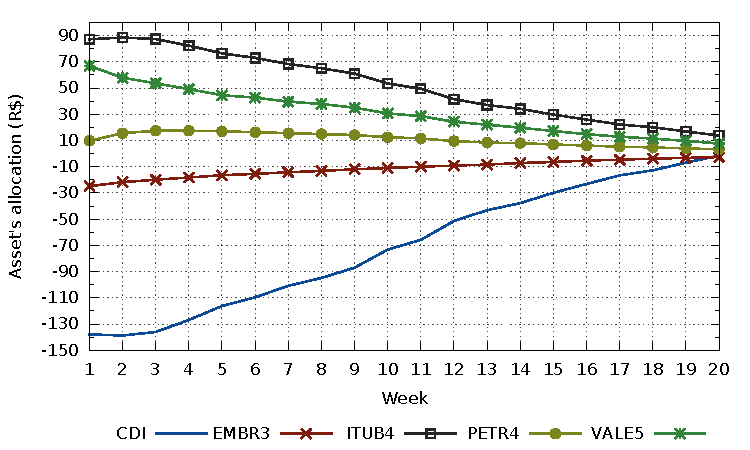
\includegraphics[width=6in,keepaspectratio]{figures/u_A}
	\source{author.}
	\label{fig:u1}
\end{figure}
%
\begin{figure} [H]
	\caption{Control policy for scenario B.}
	\centering
	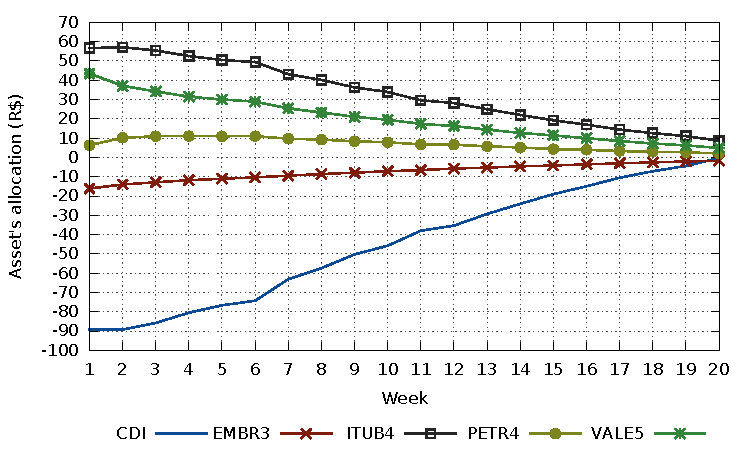
\includegraphics[width=6in,keepaspectratio]{figures/u_B}
	\source{Author.}
	\label{fig:u2}
\end{figure}
%
\begin{figure} [H]
	\caption{Control policy for scenario C.}
	\centering
	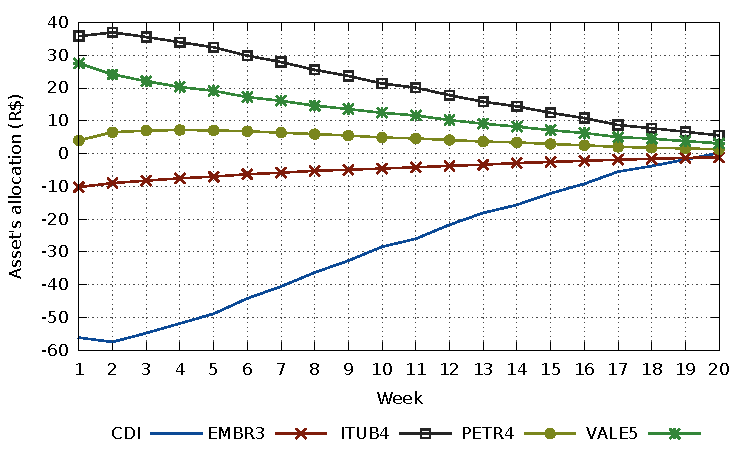
\includegraphics[width=6in,keepaspectratio]{figures/u_C}
	\source{Author.}
	\label{fig:u3}
\end{figure}
%
\begin{figure} [H]
	\caption{Control policy for scenario D.}
	\centering
	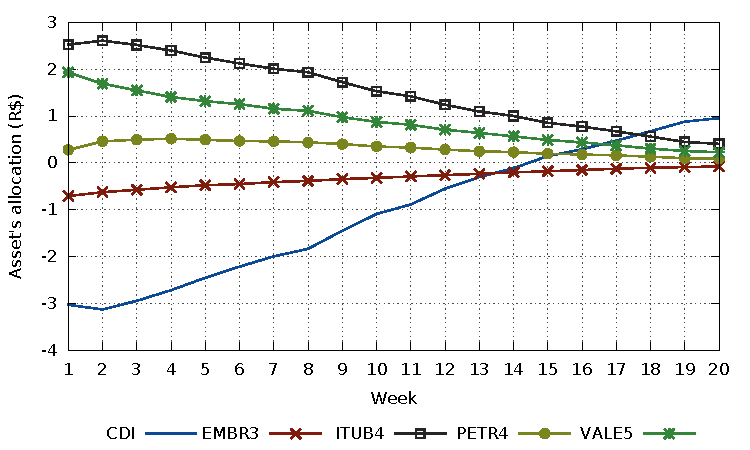
\includegraphics[width=6in,keepaspectratio]{figures/u_D}
	\source{Author.}
	\label{fig:u4}
\end{figure}
%\vspace{0pt}


% -------------------------------------###############
\subsection{Sensitivity analysis for $\beta$ and $\nu$} \label{specific}
% -------------------------------------###############


In the previous sections we described how to obtain the optimal allocation of assets in a portfolio using our results and also provided a sensitivity analysis regarding the restriction $\alpha$.
Now, our goal is to illustrate how the portfolio's value, its variance and optimal assets allocation changes with variations in one single element of both risk parameters $\beta$ and $\nu$.

In this section, we simulate an arbitrary scenario where we say the investor wishes to increase the portfolio's value around step $t=t_a$ and decrease the portfolio's volatility around another step $t=t_b$, which is achieved by adjusting the values of $\beta(t_a)$ and $\nu(t_b)$, respectively.
%
The other way around or any other combination of possible scenarios would lead to the same conclusions regarding the results' sensitivity and, therefore, were omitted in this analysis.
Nonetheless, in the Appendix \ref{app:E}, we provide further sensitivity analysis for a diverse set of combinations of possible variations between the elements of $\beta$ and $\nu$ in order to illustrate the generalization of the conclusions laid out here and summarized in the next section.

The portfolio's assets and their characteristics are the same as described earlier in Section \ref{s1}. 
In order to facilitated the comparison among all scenarios, we will solve the $PC(\nu,\beta,\alpha)$ problem for the same arbitrary restriction, $\alpha=100$, in all scenarios and run  10,000 simulations to compute the results for each of them.
%

We start with a base scenario, $cc$, where the vectors $\beta$ and $\nu$ have all unitary elements and then we apply a variation in a single element of each vector to assess their effects on the portfolio's results.
%
In order to ease the graphical observation of the variations in the results, we arbitrarily pick two specific time steps that are "sufficiently" distant from each other and, in this case, we chose $t_a=4$ and $t_b=9$.
%
Then we set "big" enough new elements for $\beta(4)$ and $\nu(9)$ in order to get visible changes in our charts.
After some try and error, we choose $\{3,5,7,9,11\}$ as the set of possible new coefficients' values for illustration purposes and label the following scenarios using the above rational, see Table \ref{tab:scenarios4}.
%
\begin{table}[h!]
	\caption{Scenarios that combine specific changes in the coefficients of $\beta$ and $\nu$ and a base scenario $cc$.}
	\centering
	\begin{tabular}{*{6}{c}}
		\specialrule{1.5pt}{2pt}{2pt}
			\multicolumn{2}{c}{}& \multicolumn{3}{c}{Input parameter} 
																& \multicolumn{1}{c}{}\\
	 	\specialrule{0.3pt}{2pt}{2pt}
	 		& & & & & Resulting \\
			Scenario & Problem applied & $\beta(4)$  & $\nu(9)$   & $\alpha$ &  $f(\beta,\alpha)$ \\
		\specialrule{0.3pt}{2pt}{2pt}
			\textbf{cc}			& $PC(\nu,\beta,\alpha)$ & \textbf{1}		& \textbf{1}	& 100 & 0.920\\
			\textbf{beta7}		& $PC(\nu,\beta,\alpha)$ & \textbf{7}		& \textbf{1} & 100 & 0.819\\
			\textbf{nu7}		& $PC(\nu,\beta,\alpha)$ & \textbf{1}		& \textbf{7} & 100 & 1.050\\
		\specialrule{0.3pt}{2pt}{2pt}
			COMBINED-3		& $PC(\nu,\beta,\alpha)$ & 3		& 3	& 100 & 0.939\\
			COMBINED-5		& $PC(\nu,\beta,\alpha)$ & 5		& 5	& 100 & 0.937\\
			\textbf{COMBINED-7}		& $PC(\nu,\beta,\alpha)$ & \textbf{7}		& \textbf{7}	& 100 & 0.925\\
			COMBINED-9		& $PC(\nu,\beta,\alpha)$ & 9		& 9	& 100 & 0.907\\
			COMBINED-11		& $PC(\nu,\beta,\alpha)$ & 11	& 11& 100 & 0.887\\
		\specialrule{1.5pt}{2pt}{2pt}
		\multicolumn{6}{c}{Note: $\beta(t)=1$ and $\nu(t)=1$ for all the remaining $t$, $t \in \{1,\cdots, 20\}-\{4,9\}$.}
	\end{tabular}
	\source{Author.}
	\label{tab:scenarios4}
\end{table}

We will focus the analysis based on four scenarios, $cc$, $beta7$, $nu7$, and $COMBINED-7$.
This will allow us to see the specific effects around the scenario $cc$ by first changing $\beta(4)$ to $7$ in scenario $beta7$, by changing $\nu(9)$ to $7$ in scenario $nu7$, and then combining the effects of both changes in scenario $COMBINED-7$.
The remaining scenarios will only be used to illustrated the sensitivity of the results of scenario $COMBINED-7$ for different levels of $\beta(4)$  and $\nu(9)$.

Figures \ref{fig:y_spec1} and \ref{fig:var_spec1} show the portfolio's value and its variance for the four scenarios described above.
As one can easily observe in the curve of $beta7$ versus $cc$, an increase in $\beta(4)$ leads to an increase in the portfolio's value from $t=1$ up to $t=4$ followed by a correspondent increase in the variance.
After $t=4$, $\beta$ decreases back to $1$ and the portfolio's value and its variance decreases.

In scenario $nu7$, we can see that an increase in $\nu(9)$ leads to a decrease in the variance from $t=3$ up to $t=9$ followed by a correspondent decrease in the portfolio's value.
%
Then, at $t=10$, $\nu$ decreases back to 1 which leads to the opposite effect just described.


Note that, given we imposed a restriction on the total variance for all scenarios, $\alpha=100$, the higher variances obtained until $t=4$ in scenario $beta7$ will be compensated with lower variances in the later periods when compared with those from the base scenario $cc$.
%
The same reasoning applies for scenario $nu7$, where the restriction $\alpha=100$ will force a compensation in the later periods leading them to show higher variances when compared with those from the base scenario $cc$.
%
The correspondent returns in the later periods will follow their variances with the same trend of higher or lower values. 
%
However, the accumulated returns will also influence the final results and it explains why scenario $beta7$ showed a higher return than the one of scenario $nu7$ after $t=10$.

As we can see in scenario $COMBINED-7$, the combined effect of $\beta(4)=7$ and $\nu(9)=7$ leads to the same trends regarding the output and its variance as stated above.
However, now there are some compensation on the final results due to the opposite effects of each variation.
 
Note that the parameters $\alpha=100$, $\beta(4)=7$, and $\nu(9)=7$ will affect all the values of the portfolio and their volatility over the whole time period, $T=20$.
However, the strongest effect of $\beta(4)$ and $\nu(9)$ are around $t=4$ and $t=9$, respectively, which means that it is possible to be specific about the desired relevance of the portfolio's value and its volatility on each time step even though we can not be specific about the combined result a priori.

It is also worth to mention that by setting a coefficient seven times higher than any other coefficient does not mean achieving a portfolio's value seven times higher or a volatility seven times lower than otherwise.
%the remaining coefficients would achieve.
In our example, the portfolio's value increased from around 5 to 6 by choosing $\beta(4)=7$, see curves $cc$ and $beta7$ in Figure \ref{fig:y_spec1} at $t=4$.

%
\begin{figure} [H]
	\caption{System's output for scenario $COMBINED-7$, $beta7$, $nu7$, and base scenario $cc$.}
	\centering
	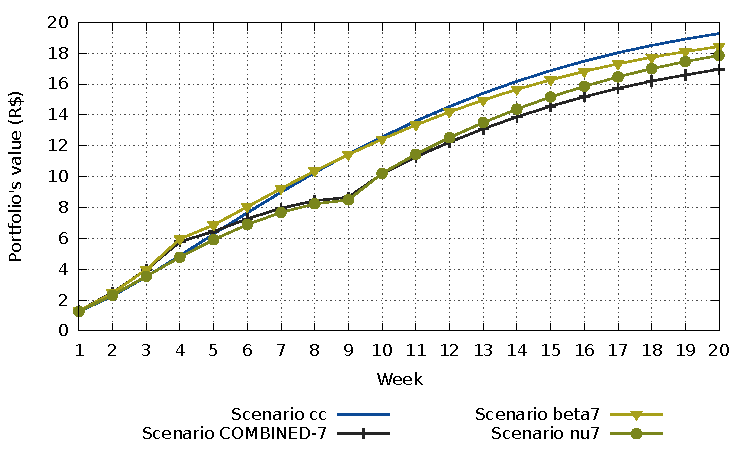
\includegraphics[width=5.9in,keepaspectratio]{figures/y_spec1}
	\source{Author.}
	\label{fig:y_spec1}
\end{figure}
%
\begin{figure} [H]
	\caption{System's output variance for scenario $COMBINED-7$, $beta7$, $nu7$, and base scenario $cc$.}
	\centering
	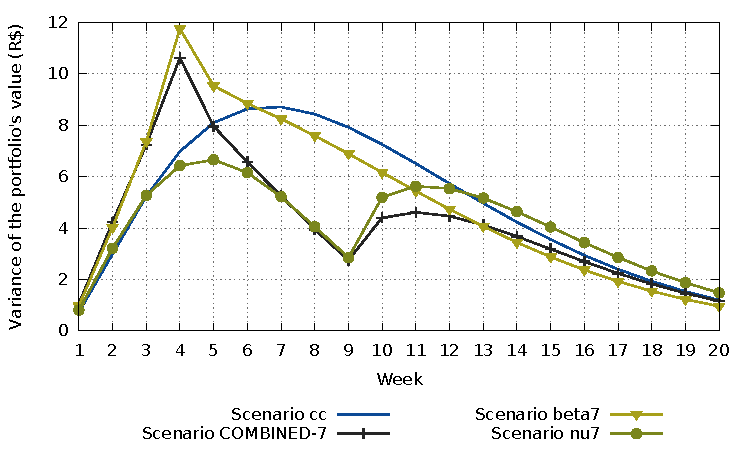
\includegraphics[width=5.9in,keepaspectratio]{figures/var_spec1}
	\source{Author.}
	\label{fig:var_spec1}
\end{figure}


Looking at the wealth allocation for scenarios $COMBINED-7$ versus $cc$ in Figure \ref{fig:u_spec1}, we can see that setting a higher expected portfolio's value through  $\beta(4)=7$ leads to an increase in the wealth allocated in the risk assets and to a lower asset allocation in the risk-free asset up to $t=4$.
In the same way, setting a lower volatility at $t=9$ through $\nu(9)=7$ forces the opposite effect on the wealth allocation.

Note that, after the point $t=9$, the asset allocation tends to the one of scenario $cc$ because the values $\beta(4)=7$ and $\nu(9)=7$ coincidentally counter-balanced each other in this short period of time. %in this example.
However, this is not necessarily true if we choose other values for $\alpha$, $\beta(t)$, and $\nu(t)$.
%
\begin{figure} [H]
	\caption{Control policy for scenario $COMBINED-7$ versus the base scenario $cc$.}
	\centering
	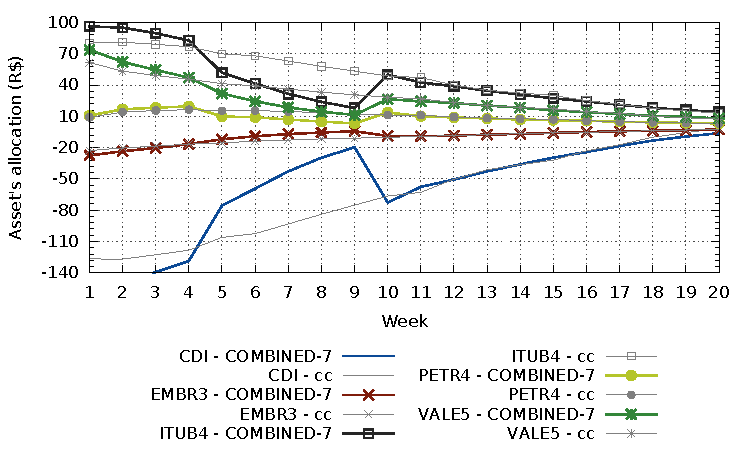
\includegraphics[width=6in,keepaspectratio]{figures/u_spec1}
	\source{Author.}
	\label{fig:u_spec1}
\end{figure}


The results for the remaining scenarios of Table \ref{tab:scenarios4} will lead to an identical conclusion to the one described above and, therefore, we will only show their results in Figures \ref{fig:y_spec56789} and \ref{fig:var_spec56789} to illustrate the sensitivity of the output and the variance around scenario $cc$ for different values of $\beta(4)$ and $\nu(9)$.
%
Note that the variations in the portfolio's value and in its variance are not proportional to the changes in the coefficients, illustrating our comments above.
%
\begin{figure} [H]
	\caption{System's output for scenario COMBINED-5,6,7,8,9 and base scenario $cc$.}
	\centering
	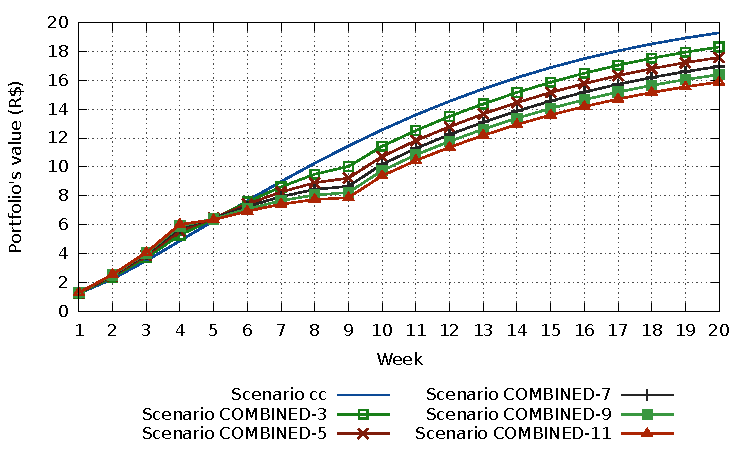
\includegraphics[width=6in,keepaspectratio]{figures/y_spec56789}
	\source{Author.}
	\label{fig:y_spec56789}
\end{figure}
%
\begin{figure} [H]
	\caption{System's output variance for scenario COMBINED-5, 6, 7, 8, 9 and base scenario $cc$.}
	\centering
	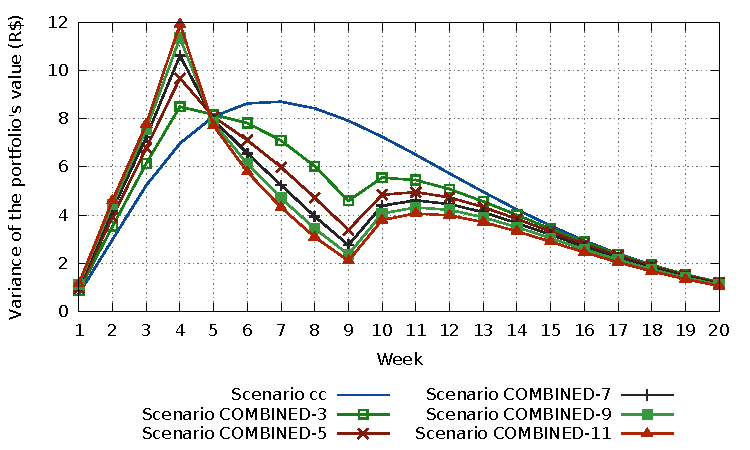
\includegraphics[width=6in,keepaspectratio]{figures/var_spec56789}
	\source{Author.}
	\label{fig:var_spec56789}
\end{figure}
\vfill


% -------------------------------------###############
\subsection{Sensitivity analysis summary and final comments} \label{sens_summary}
% -------------------------------------###############

Following the above discussion and recalling the effects of $\alpha$ from the analysis carried out in Section \ref{s_alpha}, we can summarize the effects that $\beta$, $\nu$, and $\alpha$ will have on the expected system's output, its variance, and on the wealth allocation policy, see Table \ref{tab:summary}.
%
\begin{table}[h!]
	\caption{Effects of changes in $\beta$, $\nu$, and $\alpha$ on the expected portfolio's value, its variance, and on the wealth allocation policy.}
	\centering
	\begin{tabular}{*{5}{c}}
		\specialrule{1.5pt}{2pt}{2pt}
			\multicolumn{3}{c}{} & \multicolumn{2}{c}{Wealth allocation on}\\
		\specialrule{0.3pt}{2pt}{2pt}
			Risk parameter & $E[y^u(t)]$ 	&  $Var[y^u(t)]$ & risk assets & risk-free asset \\
		\specialrule{0.3pt}{2pt}{2pt}
			$\beta(t)$ $\uparrow$		& $\uparrow$	&  $\uparrow$ 
															&  $\uparrow$ & $\downarrow$\\
			$\beta(t)$ $\downarrow$		& $\downarrow$	&  $\downarrow$ 
															& $\downarrow$ & $\uparrow$ \\
			$\nu(t)$ $\uparrow$			& $\downarrow$	&  $\downarrow$ 
															& $\downarrow$ & $\uparrow$ \\
			$\nu(t)$ $\downarrow$		& $\uparrow$	&  $\uparrow$
															&  $\uparrow$ & $\downarrow$\\
			$\alpha$ $\uparrow$			& $\uparrow$	&  $\uparrow$
															&  $\uparrow$ & $\downarrow$\\				
			$\alpha$ $\downarrow$		& $\downarrow$	&  $\downarrow$ 
															& $\downarrow$ & $\uparrow$ \\
		\specialrule{1.5pt}{2pt}{2pt}
	\end{tabular}
	\source{Author.}
	\label{tab:summary}
\end{table}

Note that these general effects are valid for variations within the elements of $\beta$ and $\nu$ as well as variations between the cross elements of those vectors.

Nonetheless, there is no standard or scientific procedure to determine the exactly coefficients that someone should use as inputs for our risk parameters.
In order to understand and recognize the investor's risk-aversion/risk-taking sentiment and the trade-offs between $\beta$, $\nu$, and $\alpha$, we suggest a similar analysis to the one developed in this chapter, where through modeling and testing different scenarios, someone would be able to understand the potential gains and losses involved and what would be the proper parameters inputs that represent his/her boundary conditions regarding returns and variances over time.

\vfill
	\chapter{Conclusion} \label{chap:conclusion}

In this work we have considered ...
	\bibliography{doc/bibliography}
		\appendix
		\chapter{bla bla} \label{app:A}

Example of long tables that cross pages.

\setstretch{1.3}

\begin{center}
\begin{longtable}{*{5}{c}}
	\caption{System's output for all scenarios.}\\
	\specialrule{1.5pt}{2pt}{2pt}
	Time	& Scenario 1	& Scenario 2	& Scenario 3	& Scenario 4 \\
	\specialrule{0.1pt}{2pt}{2pt}
	\endfirsthead

	\specialrule{1.5pt}{2pt}{2pt}
	Time	& Scenario 1	& Scenario 2	& Scenario 3	& Scenario 4 \\
	\specialrule{0.1pt}{2pt}{2pt}
	\endhead
	
	\specialrule{0.3pt}{2pt}{2pt}
	\multicolumn{5}{c}{{Continued on next page}} \\
	\specialrule{0.3pt}{2pt}{2pt}	
	\endfoot
	\endlastfoot
		
		1	& 1.3	& 1.2	& 1.1	& 1.0\\
		2	& 2.4	& 1.9	& 1.6	& 1.0\\
		3	& 3.7	& 2.8	& 2.1	& 1.1\\
		4	& 5.2	& 3.7	& 2.7	& 1.2\\
		5	& 6.7	& 4.7	& 3.4	& 1.2\\
		6	& 8.2	& 5.7	& 4.0	& 1.3\\
		7	& 9.7	& 6.7	& 4.6	& 1.3\\
		8	& 11.1	& 7.6	& 5.2	& 1.4\\
		9	& 12.4	& 8.4	& 5.7	& 1.4\\
		10	& 13.6	& 9.2	& 6.2	& 1.4\\
		11	& 14.7	& 9.9	& 6.7	& 1.5\\
		12	& 15.7	& 10.6	& 7.1	& 1.5\\
		13	& 16.7	& 11.2	& 7.5	& 1.5\\
		14	& 17.5	& 11.7	& 7.8	& 1.5\\
		15	& 18.3	& 12.2	& 8.1	& 1.6\\
		16	& 18.9	& 12.7	& 8.4	& 1.6\\
		17	& 19.5	& 13.1	& 8.6	& 1.6\\
		18	& 20.0	& 13.4	& 8.9	& 1.6\\
		19	& 20.5	& 13.7	& 9.0	& 1.6\\
		20	& 20.9	& 13.9	& 9.2	& 1.6\\
		1	& 1.3	& 1.2	& 1.1	& 1.0\\
		2	& 2.4	& 1.9	& 1.6	& 1.0\\
		3	& 3.7	& 2.8	& 2.1	& 1.1\\
		4	& 5.2	& 3.7	& 2.7	& 1.2\\
		5	& 6.7	& 4.7	& 3.4	& 1.2\\
		6	& 8.2	& 5.7	& 4.0	& 1.3\\
		7	& 9.7	& 6.7	& 4.6	& 1.3\\
		8	& 11.1	& 7.6	& 5.2	& 1.4\\
		9	& 12.4	& 8.4	& 5.7	& 1.4\\
		10	& 13.6	& 9.2	& 6.2	& 1.4\\
		11	& 14.7	& 9.9	& 6.7	& 1.5\\
		12	& 15.7	& 10.6	& 7.1	& 1.5\\
		13	& 16.7	& 11.2	& 7.5	& 1.5\\
		14	& 17.5	& 11.7	& 7.8	& 1.5\\
		15	& 18.3	& 12.2	& 8.1	& 1.6\\
		16	& 18.9	& 12.7	& 8.4	& 1.6\\
		17	& 19.5	& 13.1	& 8.6	& 1.6\\
		18	& 20.0	& 13.4	& 8.9	& 1.6\\
		19	& 20.5	& 13.7	& 9.0	& 1.6\\
		20	& 20.9	& 13.9	& 9.2	& 1.6\\
		\specialrule{0.3pt}{2pt}{2pt}	
		\multicolumn{5}{c}{Source: Author.}
\end{longtable}

\end{center}

\vfill
\setstretch{\taxaespacoduplo}
\end{document}
% =============================================================================